\documentclass[border=1pt]{standalone}
\usepackage[dvipsnames]{xcolor}
\usepackage{tikz}                       % Graphen und kommutative Diagramme
\usetikzlibrary{patterns}               % Um schraffierte Formen in der tikzpicture-Umgebung zu zeichnen.
\newcommand{\ul}[1]{\underline{\smash{#1}}}

\begin{document}
\centering
\begin{minipage}{.35\textwidth}
\centering
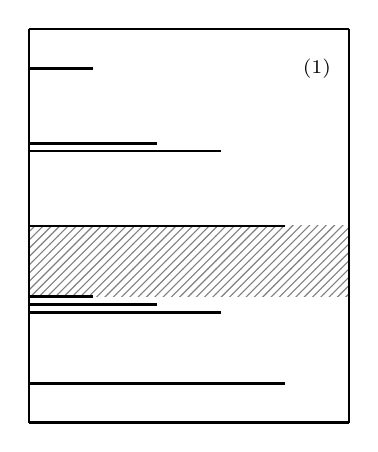
\begin{tikzpicture}[yscale=.8, xscale=.65, x=1.25cm, y=1.25cm, line width=1pt];
    \filldraw[pattern=north east lines, pattern color=gray, draw=none] (0, 2.1) -- (5, 2.1) -- (5,3) -- (0,3) -- cycle;
    
    \draw (0,0.5) -- (5,0.5);
    \draw (0,5.5) -- (5,5.5);
    \draw (0,0.5) -- (0,5.5);
    \draw (5,0.5) -- (5,5.5);
    
    \draw[line width=1pt] (0,5) to (1,5);
    \draw[line width=1pt] (0,2.10) to (1,2.10);
    
    \draw[line width=1pt] (0,4.05) to (2,4.05);
    \draw[line width=1pt] (0,2.00) to (2,2.00);
    
    \draw[line width=1pt] (0,3.95) to (3,3.95);
    \draw[line width=1pt] (0,1.90) to (3,1.90);
    
    \draw[line width=1pt] (0,3) to (4,3);
    \draw[line width=1pt] (0,1) to (4,1);
    
    \draw node at (4.5,5) {$\scriptstyle (1)$};
\end{tikzpicture}
\end{minipage}
\hspace{.25cm}
\begin{minipage}{.35\textwidth}
\centering
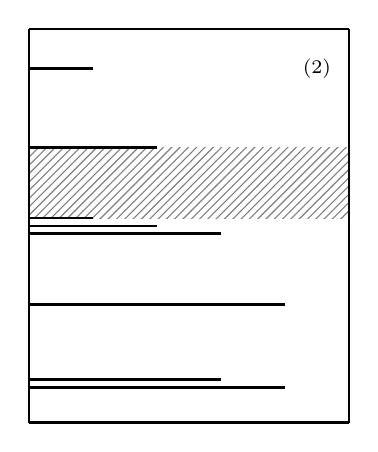
\begin{tikzpicture}[yscale=.8, xscale=.65, x=1.25cm, y=1.25cm, line width=1pt];
    \filldraw[pattern=north east lines, pattern color=gray, draw=none] (0, 4.00) -- (5, 4.00) -- (5,3.10) -- (0,3.10) -- cycle;
    
    \draw (0,0.5) -- (5,0.5);
    \draw (0,5.5) -- (5,5.5);
    \draw (0,0.5) -- (0,5.5);
    \draw (5,0.5) -- (5,5.5);
    
    \draw[line width=1pt] (0,5) to (1,5);
    \draw[line width=1pt] (0,3.10) to (1,3.10);
    
    \draw[line width=1pt] (0,4.00) to (2,4.00);
    \draw[line width=1pt] (0,3.00) to (2,3.00);
    
    \draw[line width=1pt] (0,2.90) to (3,2.90);
    \draw[line width=1pt] (0,1.05) to (3,1.05);
    
    \draw[line width=1pt] (0,2.00) to (4,2.00);
    \draw[line width=1pt] (0,0.95) to (4,0.95);
    
    \draw node at (4.5,5) {$\scriptstyle (2)$};
\end{tikzpicture}
\end{minipage}
\hspace{.25cm}
\begin{minipage}{.35\textwidth}
\centering
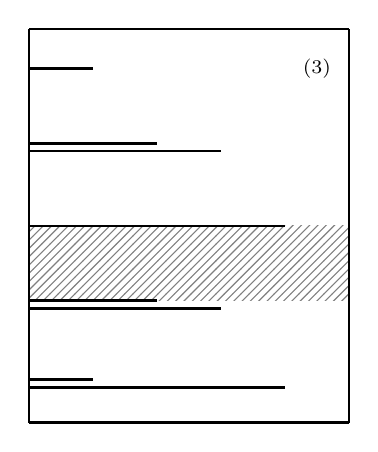
\begin{tikzpicture}[yscale=.8, xscale=.65, x=1.25cm, y=1.25cm, line width=1pt];
    \filldraw[pattern=north east lines, pattern color=gray, draw=none] (0, 2.05) -- (5, 2.05) -- (5,3) -- (0,3) -- cycle;
    
    \draw (0,0.5) -- (5,0.5);
    \draw (0,5.5) -- (5,5.5);
    \draw (0,0.5) -- (0,5.5);
    \draw (5,0.5) -- (5,5.5);
    
    \draw[line width=1pt] (0,5) to (1,5);
    \draw[line width=1pt] (0,1.05) to (1,1.05);
    
    \draw[line width=1pt] (0,4.05) to (2,4.05);
    \draw[line width=1pt] (0,2.05) to (2,2.05);
    
    \draw[line width=1pt] (0,3.95) to (3,3.95);
    \draw[line width=1pt] (0,1.95) to (3,1.95);
    
    \draw[line width=1pt] (0,3) to (4,3);
    \draw[line width=1pt] (0,0.95) to (4,0.95);
    
    \draw node at (4.5,5) {$\scriptstyle (3)$};
\end{tikzpicture}
\end{minipage}
\end{document}